% Options for packages loaded elsewhere
\PassOptionsToPackage{unicode}{hyperref}
\PassOptionsToPackage{hyphens}{url}
%
\documentclass[
]{article}
\usepackage{amsmath,amssymb}
\usepackage{iftex}
\ifPDFTeX
  \usepackage[T1]{fontenc}
  \usepackage[utf8]{inputenc}
  \usepackage{textcomp} % provide euro and other symbols
\else % if luatex or xetex
  \usepackage{unicode-math} % this also loads fontspec
  \defaultfontfeatures{Scale=MatchLowercase}
  \defaultfontfeatures[\rmfamily]{Ligatures=TeX,Scale=1}
\fi
\usepackage{lmodern}
\ifPDFTeX\else
  % xetex/luatex font selection
\fi
% Use upquote if available, for straight quotes in verbatim environments
\IfFileExists{upquote.sty}{\usepackage{upquote}}{}
\IfFileExists{microtype.sty}{% use microtype if available
  \usepackage[]{microtype}
  \UseMicrotypeSet[protrusion]{basicmath} % disable protrusion for tt fonts
}{}
\makeatletter
\@ifundefined{KOMAClassName}{% if non-KOMA class
  \IfFileExists{parskip.sty}{%
    \usepackage{parskip}
  }{% else
    \setlength{\parindent}{0pt}
    \setlength{\parskip}{6pt plus 2pt minus 1pt}}
}{% if KOMA class
  \KOMAoptions{parskip=half}}
\makeatother
\usepackage{xcolor}
\usepackage[margin=1in]{geometry}
\usepackage{color}
\usepackage{fancyvrb}
\newcommand{\VerbBar}{|}
\newcommand{\VERB}{\Verb[commandchars=\\\{\}]}
\DefineVerbatimEnvironment{Highlighting}{Verbatim}{commandchars=\\\{\}}
% Add ',fontsize=\small' for more characters per line
\usepackage{framed}
\definecolor{shadecolor}{RGB}{248,248,248}
\newenvironment{Shaded}{\begin{snugshade}}{\end{snugshade}}
\newcommand{\AlertTok}[1]{\textcolor[rgb]{0.94,0.16,0.16}{#1}}
\newcommand{\AnnotationTok}[1]{\textcolor[rgb]{0.56,0.35,0.01}{\textbf{\textit{#1}}}}
\newcommand{\AttributeTok}[1]{\textcolor[rgb]{0.13,0.29,0.53}{#1}}
\newcommand{\BaseNTok}[1]{\textcolor[rgb]{0.00,0.00,0.81}{#1}}
\newcommand{\BuiltInTok}[1]{#1}
\newcommand{\CharTok}[1]{\textcolor[rgb]{0.31,0.60,0.02}{#1}}
\newcommand{\CommentTok}[1]{\textcolor[rgb]{0.56,0.35,0.01}{\textit{#1}}}
\newcommand{\CommentVarTok}[1]{\textcolor[rgb]{0.56,0.35,0.01}{\textbf{\textit{#1}}}}
\newcommand{\ConstantTok}[1]{\textcolor[rgb]{0.56,0.35,0.01}{#1}}
\newcommand{\ControlFlowTok}[1]{\textcolor[rgb]{0.13,0.29,0.53}{\textbf{#1}}}
\newcommand{\DataTypeTok}[1]{\textcolor[rgb]{0.13,0.29,0.53}{#1}}
\newcommand{\DecValTok}[1]{\textcolor[rgb]{0.00,0.00,0.81}{#1}}
\newcommand{\DocumentationTok}[1]{\textcolor[rgb]{0.56,0.35,0.01}{\textbf{\textit{#1}}}}
\newcommand{\ErrorTok}[1]{\textcolor[rgb]{0.64,0.00,0.00}{\textbf{#1}}}
\newcommand{\ExtensionTok}[1]{#1}
\newcommand{\FloatTok}[1]{\textcolor[rgb]{0.00,0.00,0.81}{#1}}
\newcommand{\FunctionTok}[1]{\textcolor[rgb]{0.13,0.29,0.53}{\textbf{#1}}}
\newcommand{\ImportTok}[1]{#1}
\newcommand{\InformationTok}[1]{\textcolor[rgb]{0.56,0.35,0.01}{\textbf{\textit{#1}}}}
\newcommand{\KeywordTok}[1]{\textcolor[rgb]{0.13,0.29,0.53}{\textbf{#1}}}
\newcommand{\NormalTok}[1]{#1}
\newcommand{\OperatorTok}[1]{\textcolor[rgb]{0.81,0.36,0.00}{\textbf{#1}}}
\newcommand{\OtherTok}[1]{\textcolor[rgb]{0.56,0.35,0.01}{#1}}
\newcommand{\PreprocessorTok}[1]{\textcolor[rgb]{0.56,0.35,0.01}{\textit{#1}}}
\newcommand{\RegionMarkerTok}[1]{#1}
\newcommand{\SpecialCharTok}[1]{\textcolor[rgb]{0.81,0.36,0.00}{\textbf{#1}}}
\newcommand{\SpecialStringTok}[1]{\textcolor[rgb]{0.31,0.60,0.02}{#1}}
\newcommand{\StringTok}[1]{\textcolor[rgb]{0.31,0.60,0.02}{#1}}
\newcommand{\VariableTok}[1]{\textcolor[rgb]{0.00,0.00,0.00}{#1}}
\newcommand{\VerbatimStringTok}[1]{\textcolor[rgb]{0.31,0.60,0.02}{#1}}
\newcommand{\WarningTok}[1]{\textcolor[rgb]{0.56,0.35,0.01}{\textbf{\textit{#1}}}}
\usepackage{graphicx}
\makeatletter
\def\maxwidth{\ifdim\Gin@nat@width>\linewidth\linewidth\else\Gin@nat@width\fi}
\def\maxheight{\ifdim\Gin@nat@height>\textheight\textheight\else\Gin@nat@height\fi}
\makeatother
% Scale images if necessary, so that they will not overflow the page
% margins by default, and it is still possible to overwrite the defaults
% using explicit options in \includegraphics[width, height, ...]{}
\setkeys{Gin}{width=\maxwidth,height=\maxheight,keepaspectratio}
% Set default figure placement to htbp
\makeatletter
\def\fps@figure{htbp}
\makeatother
\setlength{\emergencystretch}{3em} % prevent overfull lines
\providecommand{\tightlist}{%
  \setlength{\itemsep}{0pt}\setlength{\parskip}{0pt}}
\setcounter{secnumdepth}{-\maxdimen} % remove section numbering
\ifLuaTeX
  \usepackage{selnolig}  % disable illegal ligatures
\fi
\usepackage{bookmark}
\IfFileExists{xurl.sty}{\usepackage{xurl}}{} % add URL line breaks if available
\urlstyle{same}
\hypersetup{
  pdftitle={Public Transport Winterbottlenecks},
  pdfauthor={Leonard, Stefan, Pascal},
  hidelinks,
  pdfcreator={LaTeX via pandoc}}

\title{Public Transport Winterbottlenecks}
\usepackage{etoolbox}
\makeatletter
\providecommand{\subtitle}[1]{% add subtitle to \maketitle
  \apptocmd{\@title}{\par {\large #1 \par}}{}{}
}
\makeatother
\subtitle{\href{https://github.com/paACode/publictransport_winterbottlenecks_palest}{Public
GitHub Repository}}
\author{Leonard, Stefan, Pascal}
\date{24.03.2025}

\begin{document}
\maketitle

{
\setcounter{tocdepth}{3}
\tableofcontents
}
\begin{Shaded}
\begin{Highlighting}[]
\NormalTok{a}\OtherTok{=} \DecValTok{5}
\FunctionTok{print}\NormalTok{(a)}
\end{Highlighting}
\end{Shaded}

\begin{verbatim}
## [1] 5
\end{verbatim}

\begin{Shaded}
\begin{Highlighting}[]
\NormalTok{a}\OtherTok{=} \DecValTok{5}
\FunctionTok{print}\NormalTok{(a)}
\end{Highlighting}
\end{Shaded}

\begin{verbatim}
## [1] 5
\end{verbatim}

\begin{Shaded}
\begin{Highlighting}[]
\NormalTok{a}\OtherTok{=} \DecValTok{5}
\FunctionTok{print}\NormalTok{(a)}
\end{Highlighting}
\end{Shaded}

\begin{verbatim}
## [1] 5
\end{verbatim}

\section{Generalised Additive Models
GAM}\label{generalised-additive-models-gam}

In this project, we apply Generalized Additive Models (GAMs) to analyze
the effects of various predictors on train delays, specifically focusing
on the response variables ANKUNFTDELAY\_min (arrival delay in minutes)
and ABFAHRTDELAY\_min (departure delay in minutes). Due to the limited
availability of continuous variables in our dataset these two delay
metrics will be the response variables we will focus on. A key subset of
our predictors is related to weather conditions. However, because the ZB
Bahn railway line spans multiple climatic regions, comparing
weather-related predictors across all stations introduces variability
that may obscure meaningful patterns. To address this, we restrict our
analysis to a subset of stations located within the Lucerne region,
where the climate is more uniform. This allows for a more reliable
interpretation of the relationship between weather conditions and train
delays.

\begin{Shaded}
\begin{Highlighting}[]
\CommentTok{\# General codes}
\FunctionTok{library}\NormalTok{(dplyr)}
\FunctionTok{library}\NormalTok{(ggplot2)}
\FunctionTok{library}\NormalTok{(mgcv)}
\FunctionTok{library}\NormalTok{(tidyr)}
\FunctionTok{library}\NormalTok{(caret)}


\CommentTok{\#Creating subset}

\NormalTok{zb\_final }\OtherTok{\textless{}{-}} \FunctionTok{read.csv}\NormalTok{(}\StringTok{"zentrahlbahn\_final.csv"}\NormalTok{, }\AttributeTok{header =} \ConstantTok{TRUE}\NormalTok{, }\AttributeTok{stringsAsFactors =} \ConstantTok{TRUE}\NormalTok{)}

\DocumentationTok{\#\# Subset the data}

\CommentTok{\# Define the specific Haltestellen in the region of Lucerne}
\NormalTok{haltestellen\_to\_keep }\OtherTok{\textless{}{-}} \FunctionTok{c}\NormalTok{(}\StringTok{"Luzern"}\NormalTok{, }\StringTok{"Luzern Allmend/Messe"}\NormalTok{, }\StringTok{"Kriens Mattenhof"}\NormalTok{, }\StringTok{"Horw"}\NormalTok{, }
                          \StringTok{"Hergiswil Matt"}\NormalTok{, }\StringTok{"Hergiswil NW"}\NormalTok{, }\StringTok{"Stansstad"}\NormalTok{, }\StringTok{"Stans"}\NormalTok{)}

\CommentTok{\# Subset the data}

\NormalTok{zb\_final\_subset }\OtherTok{\textless{}{-}}\NormalTok{ zb\_final }\SpecialCharTok{\%\textgreater{}\%}
  \FunctionTok{filter}\NormalTok{(HALTESTELLEN\_NAME }\SpecialCharTok{\%in\%}\NormalTok{ haltestellen\_to\_keep)}


\CommentTok{\#Removing rows NA in ANKUNFTDELAY\_min and ABFAHRTDELAY\_min}

\NormalTok{zb\_final\_subset }\OtherTok{\textless{}{-}}\NormalTok{ zb\_final\_subset }\SpecialCharTok{\%\textgreater{}\%}
  \FunctionTok{filter}\NormalTok{(}\SpecialCharTok{!}\FunctionTok{is.na}\NormalTok{(ANKUNFTDELAY\_min))}

\FunctionTok{sum}\NormalTok{(}\FunctionTok{is.na}\NormalTok{(zb\_final\_subset}\SpecialCharTok{$}\NormalTok{ANKUNFTDELAY\_min)) }\CommentTok{\#Checking if ANKUNFTDELAY\_min NA is 0}
\end{Highlighting}
\end{Shaded}

\begin{verbatim}
[1] 0
\end{verbatim}

\begin{Shaded}
\begin{Highlighting}[]
\NormalTok{zb\_final\_subset }\OtherTok{\textless{}{-}}\NormalTok{ zb\_final\_subset }\SpecialCharTok{\%\textgreater{}\%}
  \FunctionTok{filter}\NormalTok{(}\SpecialCharTok{!}\FunctionTok{is.na}\NormalTok{(ABFAHRTDELAY\_min))}

\FunctionTok{sum}\NormalTok{(}\FunctionTok{is.na}\NormalTok{(zb\_final\_subset}\SpecialCharTok{$}\NormalTok{ABFAHRTDELAY\_min)) }\CommentTok{\#Checking if ABFAHRTDELAY\_min NA is 0}
\end{Highlighting}
\end{Shaded}

\begin{verbatim}
[1] 0
\end{verbatim}

\begin{Shaded}
\begin{Highlighting}[]
\CommentTok{\#Reducing the subbset just with the relevant columns}

\NormalTok{zb\_final\_subset }\OtherTok{\textless{}{-}}\NormalTok{ zb\_final\_subset }\SpecialCharTok{\%\textgreater{}\%} \FunctionTok{select}\NormalTok{(BETRIEBSTAG, LINIEN\_TEXT, HALTESTELLEN\_NAME, ANKUNFTSZEIT, AN\_PROGNOSE, ABFAHRTSZEIT, AB\_PROGNOSE, ABFAHRTDELAY\_min, ANKUNFTDELAY\_min, Delay\_Category, TAGESZEIT, RUSH\_HOUR, w\_precip\_mm\_Luzern, w\_temp\_avg\_c\_Luzern)}
\end{Highlighting}
\end{Shaded}

R assumes for GAM models usually the gaussian family for the response
variables. Therefore, let's have a look if the response variables
ANKUNFTDELAY\_min and ABFAHRTDELAY\_min are gaussian distributed.

\begin{Shaded}
\begin{Highlighting}[]
\FunctionTok{par}\NormalTok{(}\AttributeTok{mfrow =} \FunctionTok{c}\NormalTok{(}\DecValTok{1}\NormalTok{, }\DecValTok{2}\NormalTok{))}


\FunctionTok{hist}\NormalTok{(zb\_final\_subset}\SpecialCharTok{$}\NormalTok{ANKUNFTDELAY\_min, }\AttributeTok{main =} \StringTok{"Histogram of ANKUNFTDELAY\_min"}\NormalTok{, }\AttributeTok{xlab =} \StringTok{"ANKUNFTDELAY\_min"}\NormalTok{, }\AttributeTok{col =} \StringTok{"lightblue"}\NormalTok{, }\AttributeTok{breaks =} \DecValTok{100}\NormalTok{, }\AttributeTok{xlim =} \FunctionTok{c}\NormalTok{(}\SpecialCharTok{{-}}\DecValTok{2}\NormalTok{,}\DecValTok{8}\NormalTok{))}


\FunctionTok{hist}\NormalTok{(zb\_final\_subset}\SpecialCharTok{$}\NormalTok{ABFAHRTDELAY\_min, }\AttributeTok{main =} \StringTok{"Histogram of ABFAHRTDELAY\_min"}\NormalTok{, }\AttributeTok{xlab =} \StringTok{"ABFAHRTDELAY\_min"}\NormalTok{, }\AttributeTok{col =} \StringTok{"lightblue"}\NormalTok{, }\AttributeTok{breaks =} \DecValTok{100}\NormalTok{, }\AttributeTok{xlim =} \FunctionTok{c}\NormalTok{(}\SpecialCharTok{{-}}\DecValTok{2}\NormalTok{,}\DecValTok{8}\NormalTok{))}
\end{Highlighting}
\end{Shaded}

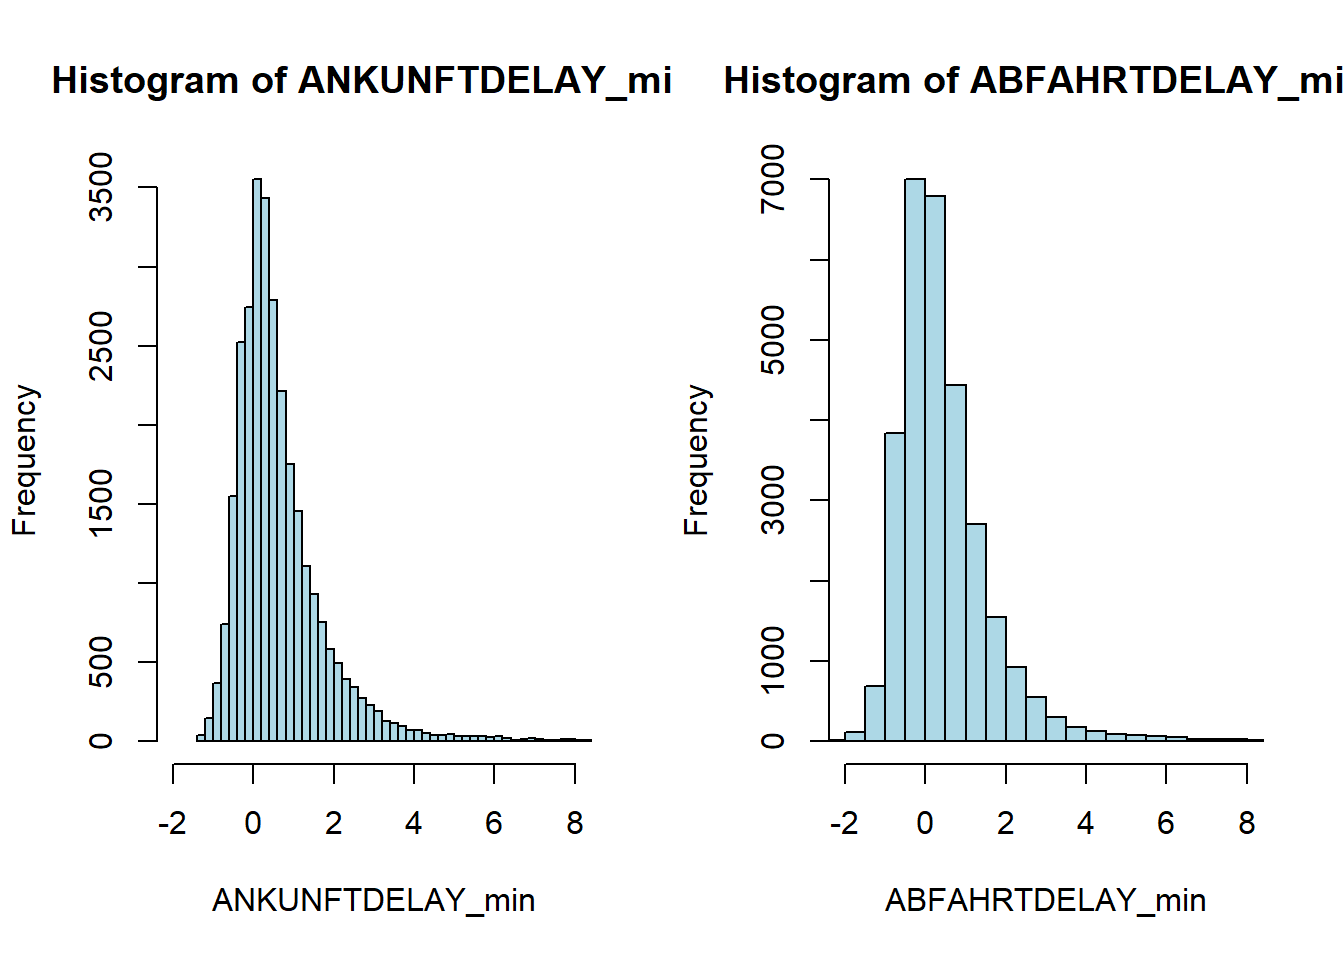
\includegraphics{final_documentation_files/figure-latex/first-histogram-1.pdf}

We see that both response variables are not normally distributed They
seem to be right skewed. Lets check with the QQ plots.

\begin{Shaded}
\begin{Highlighting}[]
\FunctionTok{par}\NormalTok{(}\AttributeTok{mfrow =} \FunctionTok{c}\NormalTok{(}\DecValTok{1}\NormalTok{, }\DecValTok{2}\NormalTok{))}

\FunctionTok{qqnorm}\NormalTok{(zb\_final}\SpecialCharTok{$}\NormalTok{ANKUNFTDELAY\_min, }\AttributeTok{main =} \StringTok{"QQ Plot of ANKUNFTDELAY\_min"}\NormalTok{)}
\FunctionTok{qqline}\NormalTok{(zb\_final}\SpecialCharTok{$}\NormalTok{ANKUNFTDELAY\_min, }\AttributeTok{col =} \StringTok{"lightblue"}\NormalTok{)}

\FunctionTok{qqnorm}\NormalTok{(zb\_final\_subset}\SpecialCharTok{$}\NormalTok{ABFAHRTDELAY\_min, }\AttributeTok{main =} \StringTok{"QQ Plot of ABFAHRTDELAY\_min"}\NormalTok{)}
\FunctionTok{qqline}\NormalTok{(zb\_final\_subset}\SpecialCharTok{$}\NormalTok{ABFAHRTDELAY\_min, }\AttributeTok{col =} \StringTok{"lightblue"}\NormalTok{)}
\end{Highlighting}
\end{Shaded}

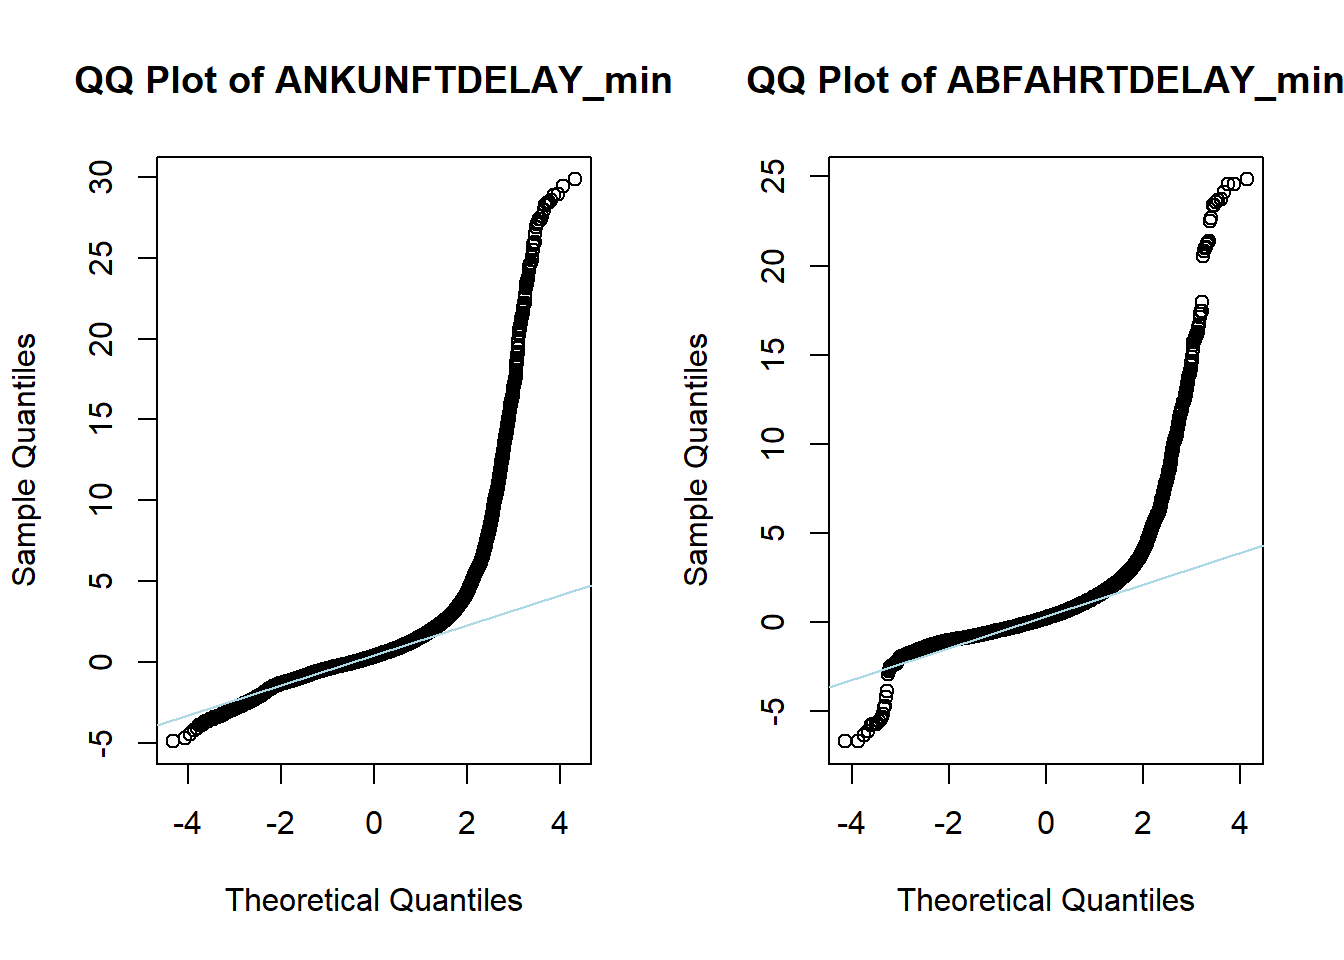
\includegraphics{final_documentation_files/figure-latex/first-qqplot-1.pdf}

The QQ plots reveal that the response variables are right-skewed, which
aligns with expectations. In real-world train operations, early arrivals
or departures are relatively uncommon compared to delays. Moreover, the
distribution indicates that longer delays occur less frequently than
shorter ones, reflecting typical delay patterns observed in Swiss public
transportation. For this reason, we restrict our dataset for the GAM
analysis to observations with delays between -2 and +4 minutes, aiming
to ensure a distribution that more closely approximates the Gaussian
assumption required by the model.

\begin{Shaded}
\begin{Highlighting}[]
\FunctionTok{par}\NormalTok{(}\AttributeTok{mfrow =} \FunctionTok{c}\NormalTok{(}\DecValTok{1}\NormalTok{, }\DecValTok{2}\NormalTok{))}

\NormalTok{zb\_final\_subset }\OtherTok{\textless{}{-}}\NormalTok{ zb\_final\_subset }\SpecialCharTok{\%\textgreater{}\%}
  \FunctionTok{filter}\NormalTok{(ABFAHRTDELAY\_min }\SpecialCharTok{\textgreater{}=} \SpecialCharTok{{-}}\DecValTok{2} \SpecialCharTok{\&}\NormalTok{ ABFAHRTDELAY\_min }\SpecialCharTok{\textless{}=} \DecValTok{4}\NormalTok{,}
\NormalTok{         ANKUNFTDELAY\_min }\SpecialCharTok{\textgreater{}=} \SpecialCharTok{{-}}\DecValTok{2} \SpecialCharTok{\&}\NormalTok{ ANKUNFTDELAY\_min }\SpecialCharTok{\textless{}=} \DecValTok{4}\NormalTok{)}


\FunctionTok{hist}\NormalTok{(zb\_final\_subset}\SpecialCharTok{$}\NormalTok{ANKUNFTDELAY\_min, }\AttributeTok{main =} \StringTok{"Histogram of ANKUNFTDELAY\_min"}\NormalTok{, }\AttributeTok{xlab =} \StringTok{"ANKUNFTDELAY\_min"}\NormalTok{, }\AttributeTok{col =} \StringTok{"lightgreen"}\NormalTok{, }\AttributeTok{breaks =} \DecValTok{50}\NormalTok{, }\AttributeTok{xlim =} \FunctionTok{c}\NormalTok{(}\SpecialCharTok{{-}}\DecValTok{2}\NormalTok{,}\DecValTok{4}\NormalTok{))}


\FunctionTok{hist}\NormalTok{(zb\_final\_subset}\SpecialCharTok{$}\NormalTok{ABFAHRTDELAY\_min, }\AttributeTok{main =} \StringTok{"Histogram of ABFAHRTDELAY\_min"}\NormalTok{, }\AttributeTok{xlab =} \StringTok{"ABFAHRTDELAY\_min"}\NormalTok{, }\AttributeTok{col =} \StringTok{"lightgreen"}\NormalTok{, }\AttributeTok{breaks =} \DecValTok{50}\NormalTok{, }\AttributeTok{xlim =} \FunctionTok{c}\NormalTok{(}\SpecialCharTok{{-}}\DecValTok{2}\NormalTok{,}\DecValTok{4}\NormalTok{))}
\end{Highlighting}
\end{Shaded}

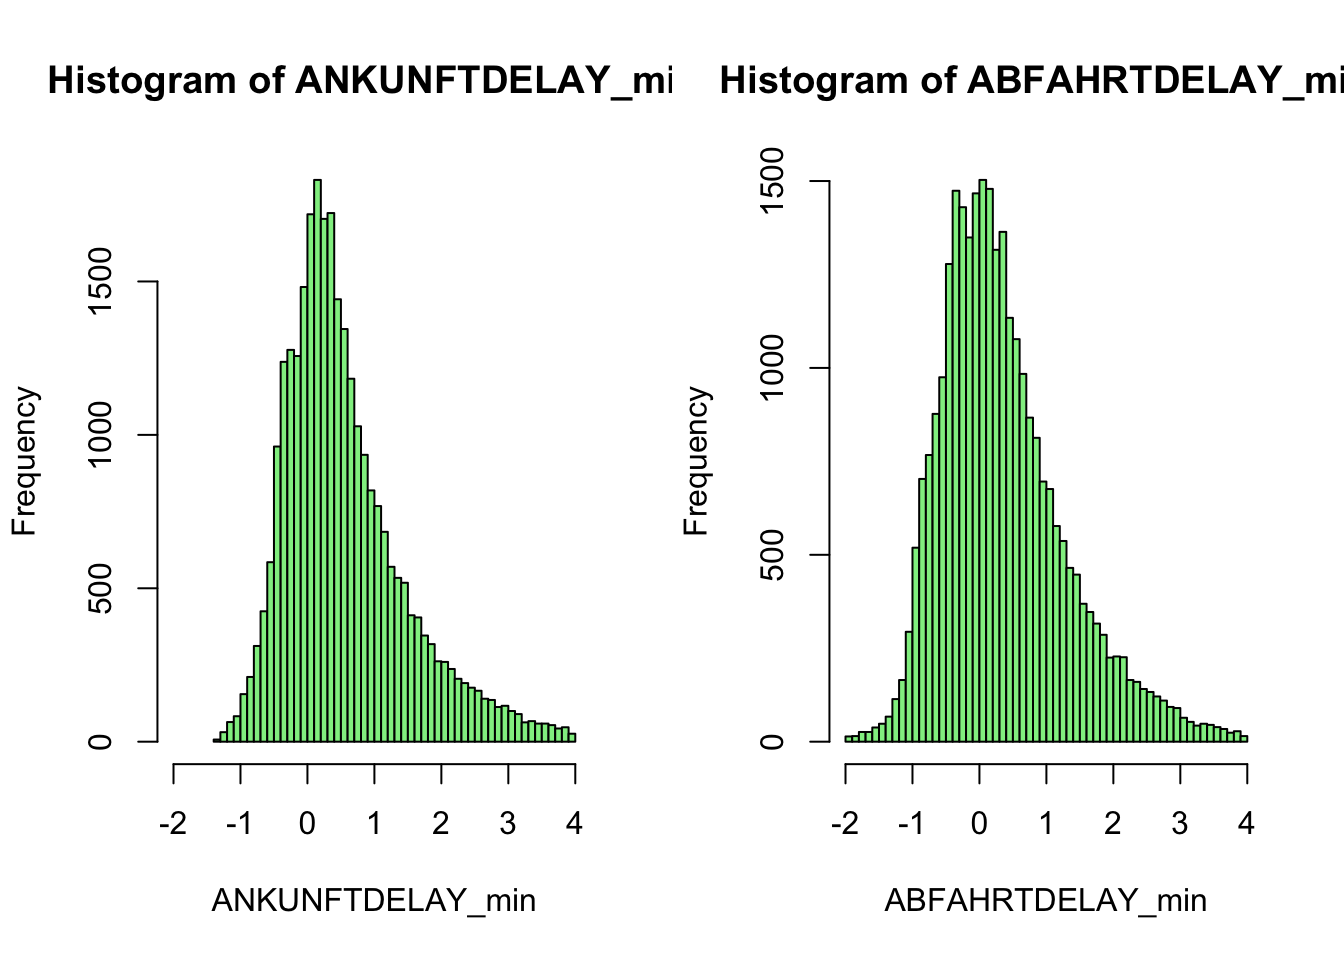
\includegraphics{final_documentation_files/figure-latex/second-histogram-1.pdf}

The histogram indicates an approximately normal distribution. Therefore,
the dataset is now suitable for fitting with Generalized Additive Models
(GAMs).

\begin{Shaded}
\begin{Highlighting}[]
\NormalTok{gam\_Ankunft\_temp }\OtherTok{\textless{}{-}} \FunctionTok{gam}\NormalTok{(ANKUNFTDELAY\_min }\SpecialCharTok{\textasciitilde{}} \FunctionTok{s}\NormalTok{(w\_temp\_avg\_c\_Luzern), }\AttributeTok{data =}\NormalTok{ zb\_final\_subset) }

\FunctionTok{summary}\NormalTok{ (gam\_Ankunft\_temp)}
\end{Highlighting}
\end{Shaded}

\begin{verbatim}

Family: gaussian 
Link function: identity 

Formula:
ANKUNFTDELAY_min ~ s(w_temp_avg_c_Luzern)

Parametric coefficients:
            Estimate Std. Error t value Pr(>|t|)    
(Intercept)  0.56586    0.00519     109   <2e-16 ***
---
Signif. codes:  0 '***' 0.001 '**' 0.01 '*' 0.05 '.' 0.1 ' ' 1

Approximate significance of smooth terms:
                         edf Ref.df   F p-value    
s(w_temp_avg_c_Luzern) 8.881  8.995 122  <2e-16 ***
---
Signif. codes:  0 '***' 0.001 '**' 0.01 '*' 0.05 '.' 0.1 ' ' 1

R-sq.(adj) =  0.0364   Deviance explained = 3.67%
GCV = 0.78087  Scale est. = 0.7806    n = 28984
\end{verbatim}

The p-value associated with the smooth term is close to zero, providing
strong evidence that the average temperature in Lucerne has a
statistically significant effect on arrival delays. The estimated
effective degrees of freedom (edf ≈ 9) suggest a moderately complex,
non-linear relationship. However, the adjusted R-squared value of 0.036
and the explained deviance of only 3.67\% indicate that the model
captures only a small portion of the variation in arrival delays. Thus,
while the effect is significant, temperature alone does not explain much
of the delay variability.

\begin{Shaded}
\begin{Highlighting}[]
\NormalTok{gam\_temp\_precip\_tageszeit\_linien\_text }\OtherTok{\textless{}{-}} \FunctionTok{gam}\NormalTok{(ABFAHRTDELAY\_min }\SpecialCharTok{\textasciitilde{}}\NormalTok{ TAGESZEIT }\SpecialCharTok{+}\NormalTok{ LINIEN\_TEXT }\SpecialCharTok{+} \FunctionTok{s}\NormalTok{(w\_temp\_avg\_c\_Luzern) }\SpecialCharTok{+} \FunctionTok{s}\NormalTok{(w\_precip\_mm\_Luzern), }\AttributeTok{data =}\NormalTok{ zb\_final\_subset) }

\FunctionTok{summary}\NormalTok{(gam\_temp\_precip\_tageszeit\_linien\_text)}
\end{Highlighting}
\end{Shaded}

\begin{verbatim}

Family: gaussian 
Link function: identity 

Formula:
ABFAHRTDELAY_min ~ TAGESZEIT + LINIEN_TEXT + s(w_temp_avg_c_Luzern) + 
    s(w_precip_mm_Luzern)

Parametric coefficients:
                    Estimate Std. Error t value Pr(>|t|)    
(Intercept)          1.24747    0.33220   3.755 0.000174 ***
TAGESZEITMittag     -0.30000    0.01880 -15.961  < 2e-16 ***
TAGESZEITNachmittag -0.16098    0.01854  -8.682  < 2e-16 ***
TAGESZEITNacht      -0.30080    0.01631 -18.441  < 2e-16 ***
TAGESZEITVormittag  -0.11592    0.01655  -7.002 2.57e-12 ***
LINIEN_TEXTIR       -0.22497    0.33290  -0.676 0.499183    
LINIEN_TEXTPE       -2.32029    0.93772  -2.474 0.013352 *  
LINIEN_TEXTS4       -0.83845    0.33198  -2.526 0.011555 *  
LINIEN_TEXTS41      -1.35328    0.33415  -4.050 5.14e-05 ***
LINIEN_TEXTS44      -1.04235    0.33382  -3.122 0.001795 ** 
LINIEN_TEXTS5       -0.50933    0.33200  -1.534 0.125008    
LINIEN_TEXTS55      -1.95525    0.33936  -5.762 8.41e-09 ***
---
Signif. codes:  0 '***' 0.001 '**' 0.01 '*' 0.05 '.' 0.1 ' ' 1

Approximate significance of smooth terms:
                         edf Ref.df     F p-value    
s(w_temp_avg_c_Luzern) 9.000  9.000 79.03  <2e-16 ***
s(w_precip_mm_Luzern)  8.319  8.591 59.29  <2e-16 ***
---
Signif. codes:  0 '***' 0.001 '**' 0.01 '*' 0.05 '.' 0.1 ' ' 1

R-sq.(adj) =  0.119   Deviance explained = 11.9%
GCV = 0.76993  Scale est. = 0.76915   n = 28984
\end{verbatim}

\begin{Shaded}
\begin{Highlighting}[]
\FunctionTok{plot}\NormalTok{(gam\_temp\_precip\_tageszeit\_linien\_text, }\AttributeTok{residuals =} \ConstantTok{TRUE}\NormalTok{, }\AttributeTok{select =} \DecValTok{1}\NormalTok{,}\AttributeTok{main =} \StringTok{"Effect of Temperature on Departure Delay"}\NormalTok{)}
\end{Highlighting}
\end{Shaded}

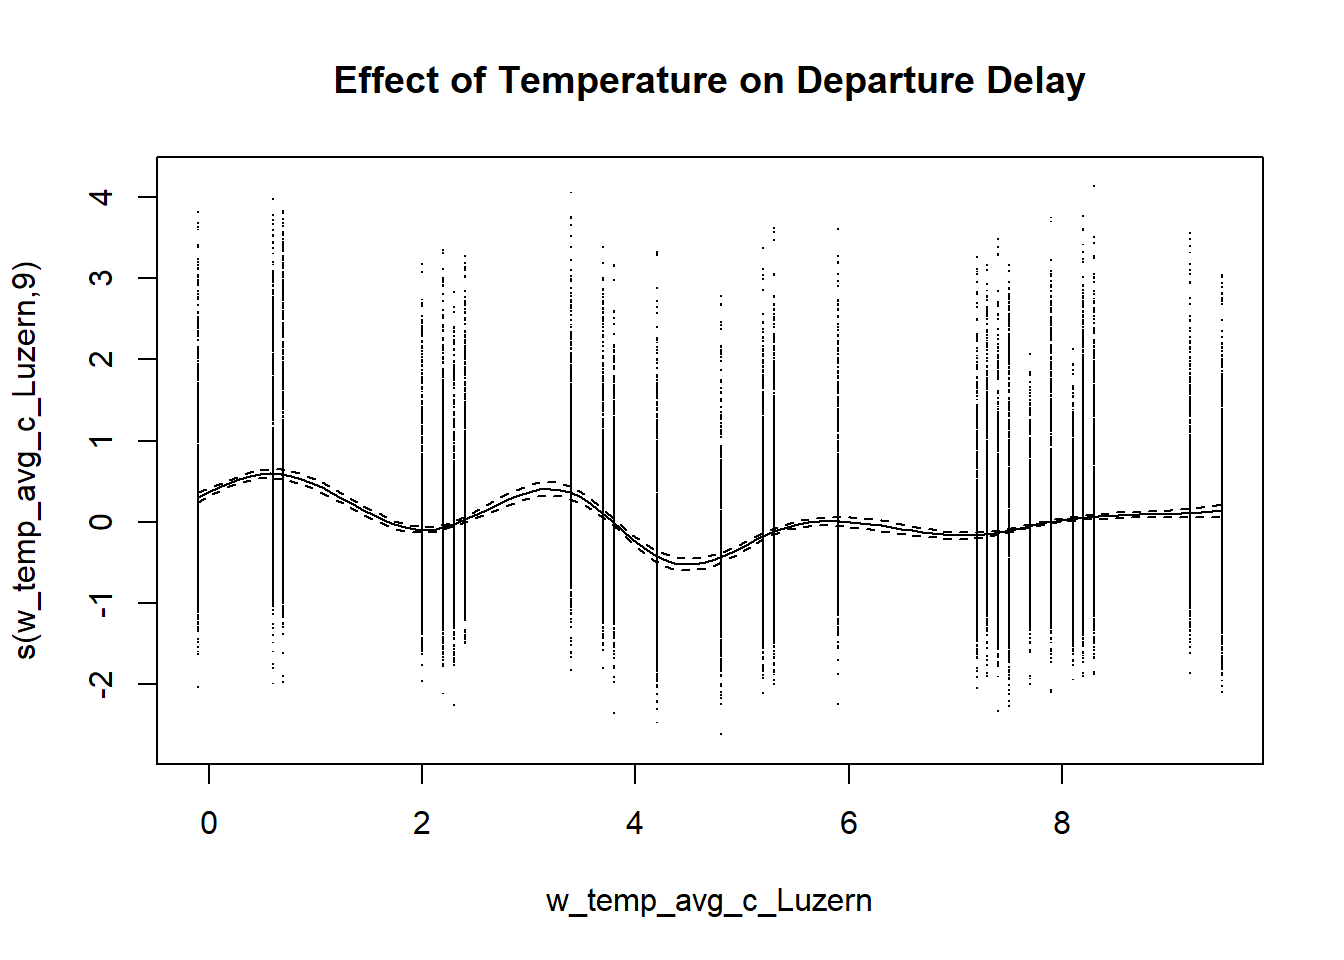
\includegraphics{final_documentation_files/figure-latex/gam-temp-precip-tageszeit-linien_text-1.pdf}

\begin{Shaded}
\begin{Highlighting}[]
\FunctionTok{plot}\NormalTok{(gam\_temp\_precip\_tageszeit\_linien\_text, }\AttributeTok{residuals =} \ConstantTok{TRUE}\NormalTok{, }\AttributeTok{select =} \DecValTok{2}\NormalTok{, }\AttributeTok{main =} \StringTok{"Effect of Precipitation on Departure Delay"}\NormalTok{)}
\end{Highlighting}
\end{Shaded}

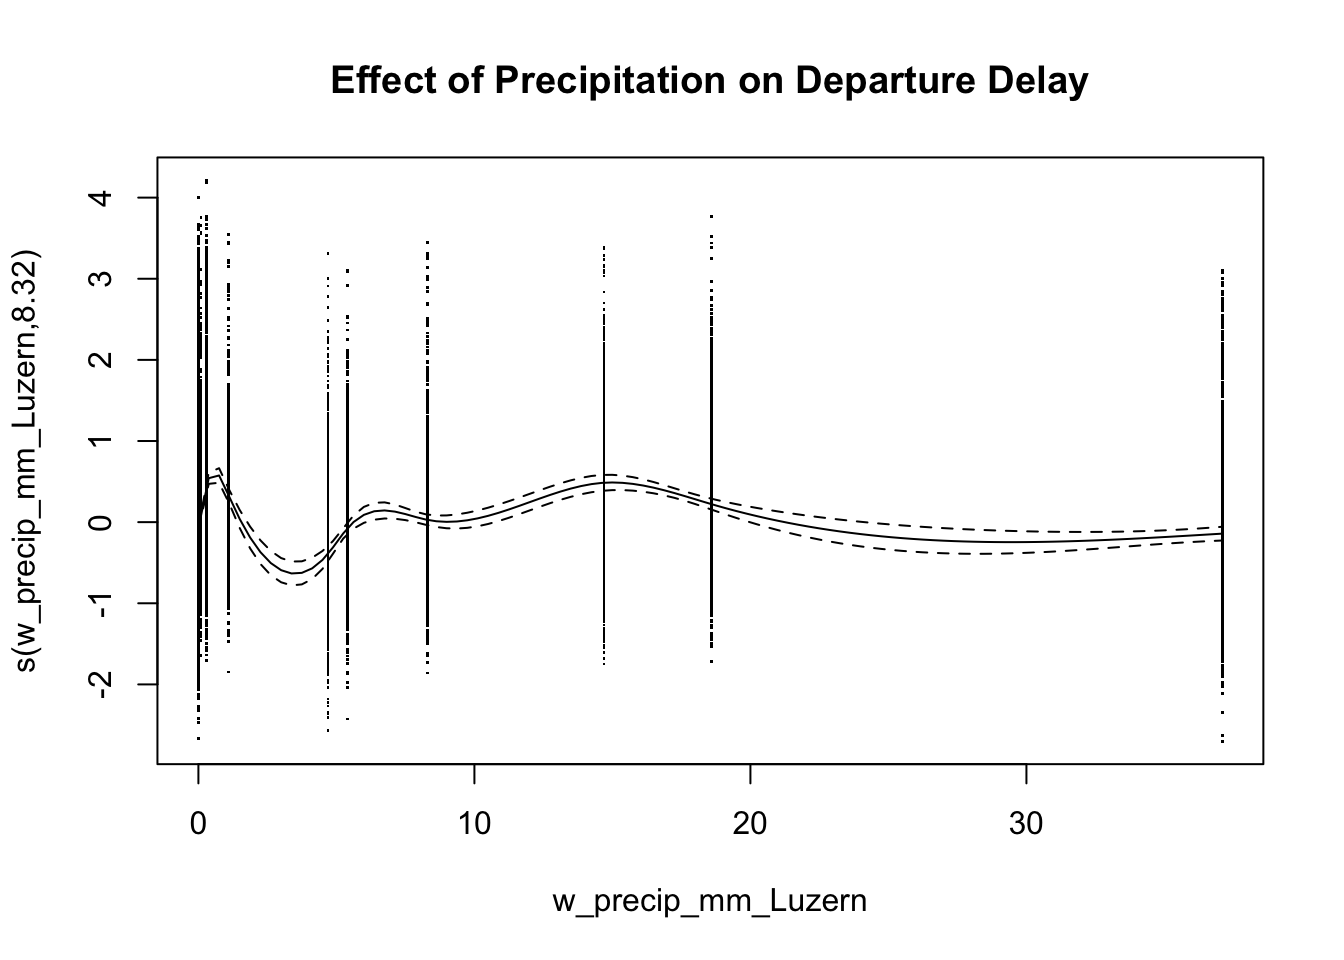
\includegraphics{final_documentation_files/figure-latex/gam-temp-precip-tageszeit-linien_text-2.pdf}

Interpretation of Parametric Coefficients The reference levels for the
categorical predictors are evening for TAGESZEIT and EXT for
LINIEN\_TEXT. Under these baseline conditions (evening, 0°C, and 0 mm
precipitation), the EXT line of Zentralbahn (ZB) in the Lucerne region
has an average departure delay of approximately 1.25 minutes.

The effect of time of day is substantial; compared to the evening,
trains during luncht time experience on average 0.30 minutes less delay,
those in the afternoon 0.16 minutes less, during night operations 0.30
minutes less and in the morning 0.12 minutes less delay.

Regarding train lines, the IR line shows a reduction of 0.22 minutes
compared to EXT, although this difference is not statistically
significant (p = 0.5). In contrast, the PE line exhibits the largest
reduction, with trains experiencing on average 2.32 minutes less delay
than EXT, a difference that is statistically significant. Likewise, the
S4, S41, S44, and S55 lines show significantly reduced delays compared
to EXT, with reductions of 0.84, 1.35, 1.04, and 1.96 minutes,
respectively, while the S5 line's difference (0.51 minutes less) is not
statistically significant.

Interpretation of the Smooth Terms The smooth term for average
temperature has an estimated effective degrees of freedom (edf) of
approximately 9, indicating a moderately complex non-linear relationship
with departure delay. We have strong evidence that it is not 0 with a
p-value \textless{} 0.05. The corresponding plot reveals that
temperatures between 0 and 6°C have a stronger effect on departure
delay, whereas between roughly 6--7°C and 8--10°C the effect is minimal.

Similarly, the smooth term for average precipitation
(w\_precip\_mm\_Luzern) has an edf of about 8.32, suggesting a
moderately complex non-linear relationship. We have strong evidence that
it is not 0 with a p-value \textless{} 0.05.

The precipitation plot shows a clear non-linear relationship between
precipitation and departure delays. There is a strong effect at lower
precipitation levels (up to approximately 20 mm), after which the curve
flattens between around 22 mm and 50 mm, indicating a reduced impact on
delays. One possible explanation for this flattening is that higher
precipitation levels may coincide with times of reduced train
activity---such as during the night---when fewer departures occur,
thereby minimizing the observed effect on overall delays. Additionally,
since the dataset only covers November 2024, it is possible that there
were relatively few instances of heavy precipitation during this period
in the Lucerne region, which may limit the model's ability to capture
stronger effects at higher precipitation levels.

Overall Model Performance The adjusted R² value of 0.119 means that the
model explains around 11.9\% of the variation in departure delays. This
suggests that the predictors included in the model have a measurable
effect on delays, but a large part of the variation (around 88\%) is
still not accounted for. This can be considered as not unusual in
real-world transportation data, where many factors that influence
delays---such as technical problems, temporary disruptions, staffing
issues or operational decisions---are not included in the dataset. While
the model successfully identifies several statistically significant
predictors, it also shows that more variables or more complex modeling
approaches might be needed to better capture all the factors that
contribute to departure delays.

\#Generalised Linear Model with family set to Binomial

\begin{Shaded}
\begin{Highlighting}[]
\NormalTok{zb\_final }\OtherTok{\textless{}{-}} \FunctionTok{read.csv}\NormalTok{(}\StringTok{"zentrahlbahn\_final.csv"}\NormalTok{, }\AttributeTok{header =} \ConstantTok{TRUE}\NormalTok{, }\AttributeTok{stringsAsFactors =} \ConstantTok{TRUE}\NormalTok{)}

\CommentTok{\#Subset}
\NormalTok{zb\_final\_binominal }\OtherTok{\textless{}{-}}\NormalTok{ zb\_final }\SpecialCharTok{\%\textgreater{}\%}
  \FunctionTok{mutate}\NormalTok{(}
    \AttributeTok{Train\_Delayed =} \FunctionTok{case\_when}\NormalTok{(}
\NormalTok{      Delay\_Category }\SpecialCharTok{==} \StringTok{"On Time"} \SpecialCharTok{\textasciitilde{}} \ConstantTok{FALSE}\NormalTok{,    }
\NormalTok{      Delay\_Category }\SpecialCharTok{==} \StringTok{"Unknown"} \SpecialCharTok{\textasciitilde{}} \ConstantTok{NA}\NormalTok{,}
\NormalTok{      Delay\_Category }\SpecialCharTok{\%in\%} \FunctionTok{c}\NormalTok{(}\StringTok{"Minor Delay"}\NormalTok{, }\StringTok{"Moderate Delay"}\NormalTok{, }\StringTok{"Significant Delay"}\NormalTok{) }\SpecialCharTok{\textasciitilde{}} \ConstantTok{TRUE}\NormalTok{,  }
      \ConstantTok{TRUE} \SpecialCharTok{\textasciitilde{}} \ConstantTok{NA}  \CommentTok{\# Handle any other unrecognized categories as NA}
\NormalTok{    ),}
    
   
    \AttributeTok{Train\_RUSH\_HOUR =} \FunctionTok{case\_when}\NormalTok{(}
\NormalTok{      RUSH\_HOUR }\SpecialCharTok{==} \StringTok{"rush\_hour\_none"} \SpecialCharTok{\textasciitilde{}} \ConstantTok{FALSE}\NormalTok{,}
\NormalTok{      RUSH\_HOUR }\SpecialCharTok{\%in\%} \FunctionTok{c}\NormalTok{(}\StringTok{"rush\_hour\_vormittag"}\NormalTok{, }\StringTok{"rush\_hour\_abend"}\NormalTok{) }\SpecialCharTok{\textasciitilde{}} \ConstantTok{TRUE}\NormalTok{,}
      \FunctionTok{is.na}\NormalTok{(RUSH\_HOUR) }\SpecialCharTok{\textasciitilde{}} \ConstantTok{NA}\NormalTok{,  }\CommentTok{\# Handle NA values properly}
      \ConstantTok{TRUE} \SpecialCharTok{\textasciitilde{}} \ConstantTok{NA}  \CommentTok{\# Any other unrecognized or unexpected RUSH\_HOUR values are NA}
\NormalTok{    )}
\NormalTok{  ) }\SpecialCharTok{\%\textgreater{}\%}
  \FunctionTok{select}\NormalTok{(}
    \DecValTok{1}\SpecialCharTok{:}\NormalTok{(}\FunctionTok{match}\NormalTok{(}\StringTok{"Delay\_Category"}\NormalTok{, }\FunctionTok{names}\NormalTok{(.))),  }\CommentTok{\# Columns up to Delay\_Category}
\NormalTok{    Train\_Delayed,  }\CommentTok{\# Add Train\_Delayed after Delay\_Category}
\NormalTok{    (}\FunctionTok{match}\NormalTok{(}\StringTok{"Delay\_Category"}\NormalTok{, }\FunctionTok{names}\NormalTok{(.)) }\SpecialCharTok{+} \DecValTok{1}\NormalTok{)}\SpecialCharTok{:}\NormalTok{(}\FunctionTok{match}\NormalTok{(}\StringTok{"RUSH\_HOUR"}\NormalTok{, }\FunctionTok{names}\NormalTok{(.))),  }\CommentTok{\# Columns between Delay\_Category and RUSH\_HOUR}
\NormalTok{    Train\_RUSH\_HOUR,  }\CommentTok{\# Add Train\_RUSH\_HOUR after RUSH\_HOUR}
\NormalTok{    (}\FunctionTok{match}\NormalTok{(}\StringTok{"RUSH\_HOUR"}\NormalTok{, }\FunctionTok{names}\NormalTok{(.)) }\SpecialCharTok{+} \DecValTok{1}\NormalTok{)}\SpecialCharTok{:}\FunctionTok{ncol}\NormalTok{(.)  }\CommentTok{\# Columns after RUSH\_HOUR}
\NormalTok{  )}

\CommentTok{\#Reducing the subset with only relevant columns}
\NormalTok{zb\_final\_binominal }\OtherTok{\textless{}{-}}\NormalTok{ zb\_final\_binominal }\SpecialCharTok{\%\textgreater{}\%} \FunctionTok{select}\NormalTok{(BETRIEBSTAG, LINIEN\_TEXT, FAELLT\_AUS\_TF, HALTESTELLEN\_NAME, ANKUNFTSZEIT, AN\_PROGNOSE, AN\_PROGNOSE\_STATUS, ABFAHRTSZEIT, AB\_PROGNOSE, AB\_PROGNOSE\_STATUS, ABFAHRTDELAY\_min, ANKUNFTDELAY\_min, Delay\_Category, Train\_Delayed, TAGESZEIT, RUSH\_HOUR, Train\_RUSH\_HOUR)}


\CommentTok{\#Removing rows NA in ANKUNFTDELAY\_min}

\NormalTok{zb\_final\_binominal }\OtherTok{\textless{}{-}}\NormalTok{ zb\_final\_binominal }\SpecialCharTok{\%\textgreater{}\%}
  \FunctionTok{filter}\NormalTok{(}\SpecialCharTok{!}\FunctionTok{is.na}\NormalTok{(ANKUNFTDELAY\_min))}

\FunctionTok{sum}\NormalTok{(}\FunctionTok{is.na}\NormalTok{(zb\_final\_binominal}\SpecialCharTok{$}\NormalTok{ANKUNFTDELAY\_min)) }\CommentTok{\#Checking if ANKUNFTDELAY\_min NA is 0}
\end{Highlighting}
\end{Shaded}

\begin{verbatim}
[1] 0
\end{verbatim}

\begin{Shaded}
\begin{Highlighting}[]
\NormalTok{zb\_final\_binominal }\OtherTok{\textless{}{-}}\NormalTok{ zb\_final\_binominal }\SpecialCharTok{\%\textgreater{}\%}
  \FunctionTok{filter}\NormalTok{(}\SpecialCharTok{!}\FunctionTok{is.na}\NormalTok{(ABFAHRTDELAY\_min))}

\FunctionTok{sum}\NormalTok{(}\FunctionTok{is.na}\NormalTok{(zb\_final\_binominal}\SpecialCharTok{$}\NormalTok{ABFAHRTDELAY\_min)) }\CommentTok{\#Checking if ABFAHRTDELAY\_min NA is 0}
\end{Highlighting}
\end{Shaded}

\begin{verbatim}
[1] 0
\end{verbatim}

\begin{Shaded}
\begin{Highlighting}[]
\CommentTok{\# Convert the Train\_Delayed to numeric (0 = FALSE, 1 = TRUE) otherwise we can not use it with a logistic regression model}
\NormalTok{zb\_final\_binominal}\SpecialCharTok{$}\NormalTok{Train\_Delayed }\OtherTok{\textless{}{-}} \FunctionTok{as.numeric}\NormalTok{(zb\_final\_binominal}\SpecialCharTok{$}\NormalTok{Train\_Delayed)}
\end{Highlighting}
\end{Shaded}

\begin{Shaded}
\begin{Highlighting}[]
\CommentTok{\#Plotting the data}

\NormalTok{zb\_final\_binominal }\SpecialCharTok{\%\textgreater{}\%}
  \FunctionTok{group\_by}\NormalTok{(LINIEN\_TEXT) }\SpecialCharTok{\%\textgreater{}\%}
  \FunctionTok{summarise}\NormalTok{(}\AttributeTok{ProportionDelayed =} \FunctionTok{mean}\NormalTok{(Train\_Delayed, }\AttributeTok{na.rm =} \ConstantTok{TRUE}\NormalTok{)) }\SpecialCharTok{\%\textgreater{}\%}
  \FunctionTok{ggplot}\NormalTok{(}\FunctionTok{aes}\NormalTok{(}\AttributeTok{x =} \FunctionTok{reorder}\NormalTok{(LINIEN\_TEXT, ProportionDelayed), }\AttributeTok{y =}\NormalTok{ ProportionDelayed)) }\SpecialCharTok{+}
  \FunctionTok{geom\_point}\NormalTok{(}\AttributeTok{size =} \DecValTok{3}\NormalTok{, }\AttributeTok{color =} \StringTok{"steelblue"}\NormalTok{) }\SpecialCharTok{+}
  \FunctionTok{labs}\NormalTok{(}\AttributeTok{x =} \StringTok{"Train Line"}\NormalTok{, }\AttributeTok{y =} \StringTok{"Proportion Delayed"}\NormalTok{) }\SpecialCharTok{+}
  \FunctionTok{theme\_minimal}\NormalTok{()}
\end{Highlighting}
\end{Shaded}

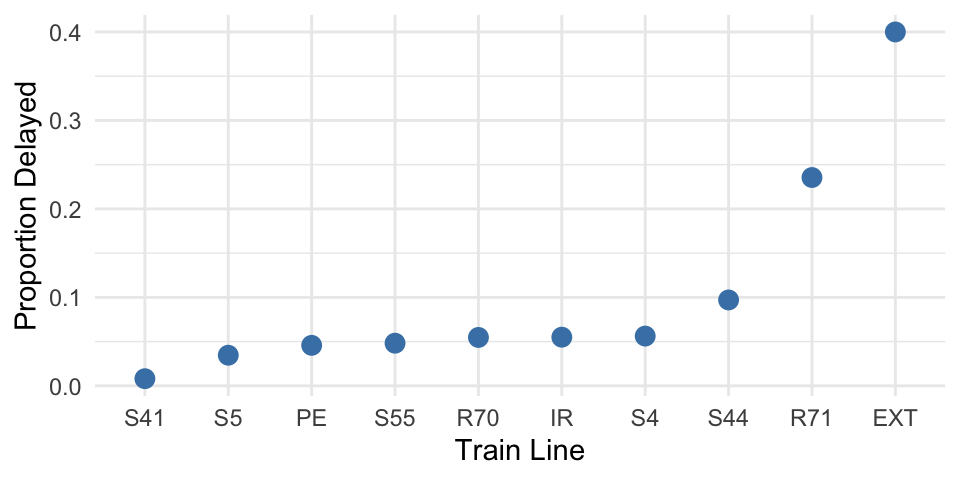
\includegraphics{final_documentation_files/figure-latex/first-plotting-1.pdf}

In this plot, we can see that the EXT line has the highest proportion of
delayed trains, with approximately 40\% of its services experiencing
delays. The line with the second highest delay rate is the R71, where
around 24\% of trains are delayed. On the other end of the spectrum, the
S41 line shows the lowest delay rate, with only about 10\% of its trains
being delayed. ''

To predict whether a train is delayed, we use a binomial logistic
regression with Train\_Delayed as the binary response variable and
LINIEN\_TEXT (train line) as the predictor. This model estimates how the
probability of delay varies across different train lines.

\begin{Shaded}
\begin{Highlighting}[]
\NormalTok{glm\_delay }\OtherTok{\textless{}{-}} \FunctionTok{glm}\NormalTok{(Train\_Delayed }\SpecialCharTok{\textasciitilde{}}\NormalTok{ LINIEN\_TEXT, }\AttributeTok{family =} \StringTok{"binomial"}\NormalTok{, }\AttributeTok{data =}\NormalTok{ zb\_final\_binominal)}

\FunctionTok{summary}\NormalTok{(glm\_delay)}
\end{Highlighting}
\end{Shaded}

\begin{verbatim}

Call:
glm(formula = Train_Delayed ~ LINIEN_TEXT, family = "binomial", 
    data = zb_final_binominal)

Coefficients:
               Estimate Std. Error z value Pr(>|z|)    
(Intercept)     -0.4055     0.6455  -0.628 0.529910    
LINIEN_TEXTIR   -2.4388     0.6489  -3.758 0.000171 ***
LINIEN_TEXTPE   -2.6321     0.6482  -4.061 4.90e-05 ***
LINIEN_TEXTR70  -2.4442     0.6551  -3.731 0.000191 ***
LINIEN_TEXTR71  -0.7723     0.6514  -1.186 0.235811    
LINIEN_TEXTS4   -2.4151     0.6464  -3.736 0.000187 ***
LINIEN_TEXTS41  -4.4067     0.8177  -5.389 7.09e-08 ***
LINIEN_TEXTS44  -1.8249     0.6584  -2.772 0.005574 ** 
LINIEN_TEXTS5   -2.9234     0.6464  -4.523 6.11e-06 ***
LINIEN_TEXTS55  -2.5777     0.6704  -3.845 0.000121 ***
---
Signif. codes:  0 '***' 0.001 '**' 0.01 '*' 0.05 '.' 0.1 ' ' 1

(Dispersion parameter for binomial family taken to be 1)

    Null deviance: 21880  on 57218  degrees of freedom
Residual deviance: 21375  on 57209  degrees of freedom
AIC: 21395

Number of Fisher Scoring iterations: 7
\end{verbatim}

The number of Fisher Scoring iterations is 7, which is an acceptable
value. The dispersion parameter in the model was calculated by dividing
the residual deviance (21375) by the residual degrees of freedom
(57209), yielding a value of 0.374. This value, being less than 1,
indicates that there is no overdispersion in the data. Therefore, the
binomial model is an appropriate fit for the dataset, and no adjustments
for overdispersion are necessary.

On one hand, the p-values for almost all the train lines are very small,
indicating that the train lines have a statistically significant effect
on whether a train is delayed or not. Since the coefficients for the
train lines are negative, it suggests that the different train lines
have a lower likeliness of being delayed compared to the baseline train
line. On the other hand, the train line R71, which operates between
Meiringen and Innertkirchen, has a p-value above 0.05. This suggests
that R71 does not have a statistically significant impact on whether a
train is delayed or not. This is interesting because, when the
predictors were plotted, R71 was the line with the second-highest
probability of delay, with an average delay of around 24\%. The reason
for this contradiction could be that while the R71 line might often
experience delays, the variance of the delays might be quite narrow. To
explore this, let's take a look at the boxplot of the train delays by
line.

\begin{Shaded}
\begin{Highlighting}[]
\FunctionTok{boxplot}\NormalTok{(ANKUNFTDELAY\_min }\SpecialCharTok{\textasciitilde{}}\NormalTok{ LINIEN\_TEXT , }\AttributeTok{data =}\NormalTok{ zb\_final\_binominal)}
\end{Highlighting}
\end{Shaded}

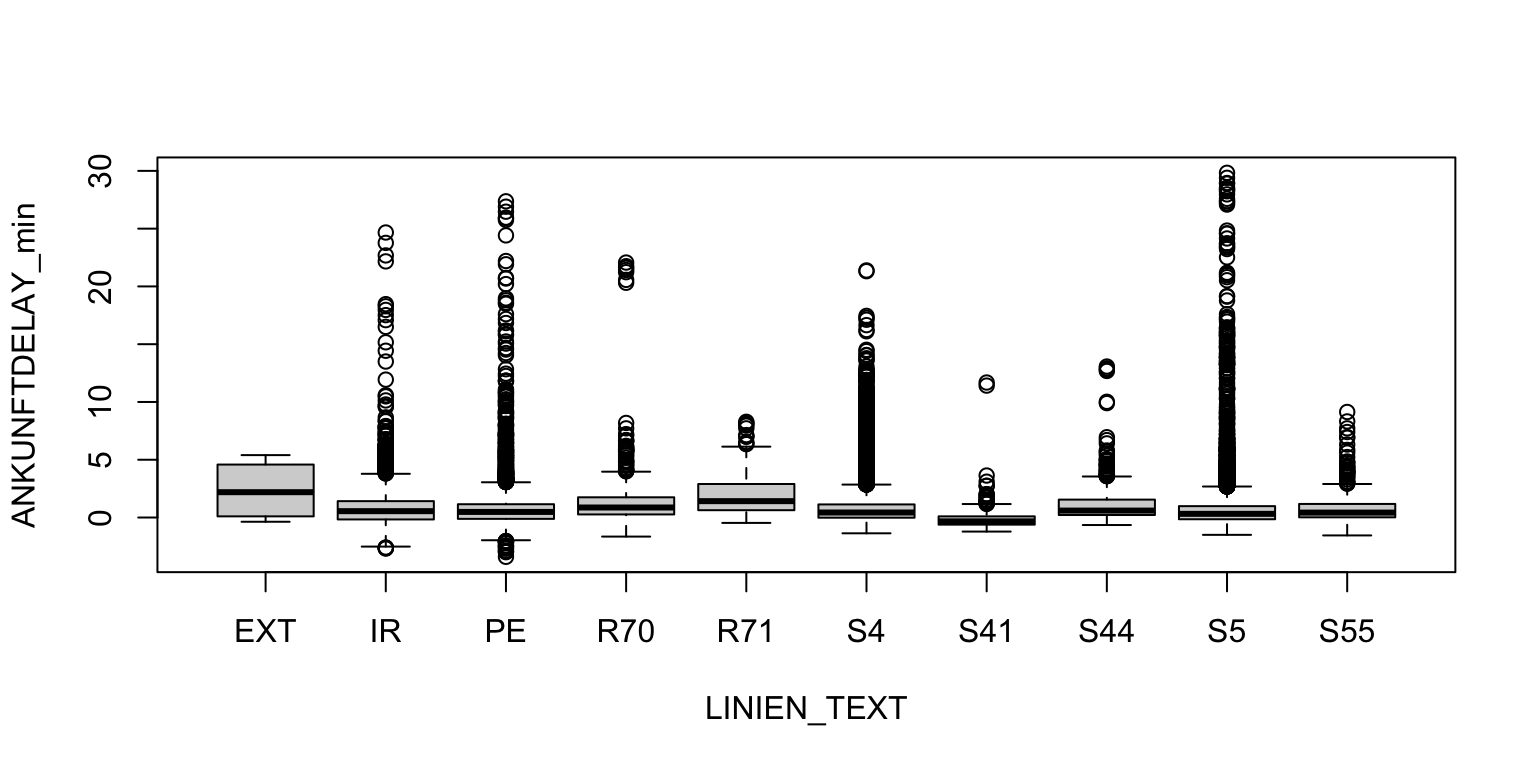
\includegraphics{final_documentation_files/figure-latex/boxplot-ANKUNFTDELAY_min-LINIEN_TEXT-1.pdf}

In the boxplot, we can see that the R71 has a relatively large variance
between the 25th and 75th percentiles of the data. Nevertheless, R71 has
fewer outliers compared to the other lines. The delays on R71 might be
consistent, but not extreme enough to be detected as a significant
predictor in the logistic regression model. Just because R71 has a
relatively high average of being delay doesn't necessarily mean that the
line itself significantly affects the likelihood of delays when
considering all other factors. The logistic regression model is trying
to predict the probability of a delay (yes/no) based on various
predictors. Other variables---such as weather, time of day, or
operational factors---might influence whether a delay occurs for R71
trains.

Lets have now a look at the coefficients of glm\_delay

\begin{Shaded}
\begin{Highlighting}[]
\FunctionTok{exp}\NormalTok{(}\FunctionTok{coef}\NormalTok{(glm\_delay)) }\SpecialCharTok{\%\textgreater{}\%} \FunctionTok{round}\NormalTok{(}\AttributeTok{digits=}\DecValTok{2}\NormalTok{)}
\end{Highlighting}
\end{Shaded}

\begin{verbatim}
   (Intercept)  LINIEN_TEXTIR  LINIEN_TEXTPE LINIEN_TEXTR70 LINIEN_TEXTR71 
          0.67           0.09           0.07           0.09           0.46 
 LINIEN_TEXTS4 LINIEN_TEXTS41 LINIEN_TEXTS44  LINIEN_TEXTS5 LINIEN_TEXTS55 
          0.09           0.01           0.16           0.05           0.08 
\end{verbatim}

To interpret the effect of different train lines on the likelihood of
delays, the logistic regression coefficients were exponentiated to
obtain odds ratios. These odds ratios provide a clearer understanding of
how the odds of a delay on each line compare to the baseline category,
which in this model is the train line EXT. All other train lines show
odds ratios significantly below 1, indicating a lower likelihood of
delay relative to EXT. For instance, trains on line IR have odds of
being delayed that are only 9\% of those on line EXT, while line S41
shows an even stronger reduction, with odds at just 1\%. Other notable
examples include lines PE and R70, each with odds around 7--9\% of the
baseline, and line S5, with only 5\% of the odds of a delay compared to
EXT. These findings suggest, as already seen in the previous plots, that
line EXT has a particularly high likelihood of delays, while other lines
operate with considerably greater punctuality.

The next step in our analysis involves simulating predictions based on
the logistic regression model to better understand the likelihood of
train delays. This will help us evaluate the model's performance and
gain insights into the probability of delays across different train
lines.

\begin{Shaded}
\begin{Highlighting}[]
\CommentTok{\# Set seed for reproducibility}
\FunctionTok{set.seed}\NormalTok{(}\DecValTok{123}\NormalTok{)}

\CommentTok{\# Simulate new data based on existing data\textquotesingle{}s structure (e.g., random values for LINIEN\_TEXT)}
\NormalTok{simulated\_data }\OtherTok{\textless{}{-}} \FunctionTok{data.frame}\NormalTok{(}
  \AttributeTok{LINIEN\_TEXT =} \FunctionTok{sample}\NormalTok{(}\FunctionTok{levels}\NormalTok{(zb\_final\_binominal}\SpecialCharTok{$}\NormalTok{LINIEN\_TEXT), }\DecValTok{10000}\NormalTok{, }\AttributeTok{replace =} \ConstantTok{TRUE}\NormalTok{) }\CommentTok{\#increased the n of trials in order to have higher sampling and higher probability range}
\NormalTok{)}

\CommentTok{\# Predict the probability of delay for these simulated data points}
\NormalTok{simulated\_data}\SpecialCharTok{$}\NormalTok{predicted\_prob }\OtherTok{\textless{}{-}} \FunctionTok{predict}\NormalTok{(glm\_delay, }\AttributeTok{newdata =}\NormalTok{ simulated\_data, }\AttributeTok{type =} \StringTok{"response"}\NormalTok{)}

\CommentTok{\# Show the first few rows of the simulated data}
\FunctionTok{head}\NormalTok{(simulated\_data)}
\end{Highlighting}
\end{Shaded}

\begin{verbatim}
  LINIEN_TEXT predicted_prob
1          PE     0.04575566
2          PE     0.04575566
3         S55     0.04819277
4          IR     0.05498045
5          S4     0.05622418
6         R71     0.23545706
\end{verbatim}

\begin{Shaded}
\begin{Highlighting}[]
\CommentTok{\# Plotting the simulated probabilities of train delays by train line}

\FunctionTok{ggplot}\NormalTok{(simulated\_data, }\FunctionTok{aes}\NormalTok{(}\AttributeTok{x =} \FunctionTok{reorder}\NormalTok{(LINIEN\_TEXT, predicted\_prob), }\AttributeTok{y =}\NormalTok{ predicted\_prob, }\AttributeTok{color =}\NormalTok{ LINIEN\_TEXT)) }\SpecialCharTok{+}
  \FunctionTok{geom\_jitter}\NormalTok{(}\AttributeTok{alpha =} \FloatTok{0.5}\NormalTok{, }\AttributeTok{width =} \FloatTok{0.2}\NormalTok{, }\AttributeTok{height =} \DecValTok{0}\NormalTok{) }\SpecialCharTok{+}
  \FunctionTok{labs}\NormalTok{(}\AttributeTok{x =} \StringTok{"Train Line"}\NormalTok{, }\AttributeTok{y =} \StringTok{"Simulated Probability of Delay"}\NormalTok{) }\SpecialCharTok{+}
  \FunctionTok{theme\_minimal}\NormalTok{() }\SpecialCharTok{+}
  \FunctionTok{theme}\NormalTok{(}
    \AttributeTok{axis.text.x =} \FunctionTok{element\_text}\NormalTok{(}\AttributeTok{angle =} \DecValTok{45}\NormalTok{, }\AttributeTok{hjust =} \DecValTok{1}\NormalTok{), }\CommentTok{\# Rotate x{-}axis labels}
    \AttributeTok{panel.border =} \FunctionTok{element\_blank}\NormalTok{(), }\CommentTok{\# Remove the box around the plot}
    \AttributeTok{legend.position =} \StringTok{"none"} \CommentTok{\# Remove the legend}
\NormalTok{  )}
\end{Highlighting}
\end{Shaded}

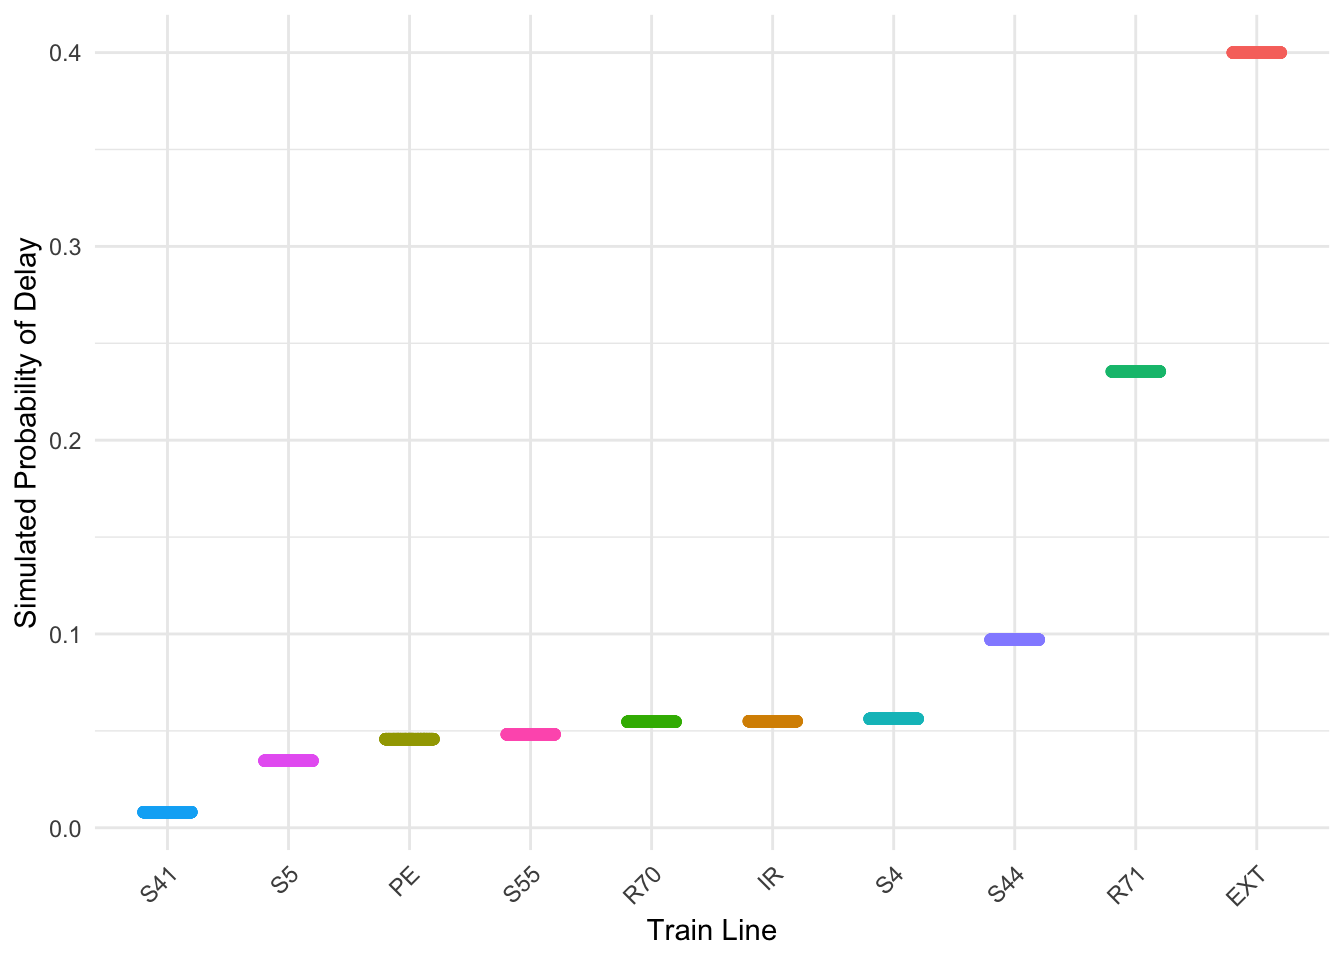
\includegraphics{final_documentation_files/figure-latex/simulation-glm-delay-1.pdf}

In this plot, we can see that the simulated data is similar to the
original data. The EXT line shows a simulated probability of delay of
approximately 40\%, while the R71 line has a simulated probability delay
of around 24\%. On the other end, the S41 line exhibits the lowest
simulated probability of delay, with only about 1\% of its services
experiencing delays.

Lets now compare our simulated data with our real dataset.

\begin{Shaded}
\begin{Highlighting}[]
\FunctionTok{summary}\NormalTok{(simulated\_data)}
\end{Highlighting}
\end{Shaded}

\begin{verbatim}
 LINIEN_TEXT        predicted_prob    
 Length:10000       Min.   :0.008065  
 Class :character   1st Qu.:0.045756  
 Mode  :character   Median :0.054980  
                    Mean   :0.104591  
                    3rd Qu.:0.097059  
                    Max.   :0.400000  
\end{verbatim}

The mean of the simulated data is 0.105. This is the reason why we
cannot take a threshold of 0.5. This would result in nearly all cases
being classified as non-delayed, since very few predicted probabilities
exceed 0.5---ultimately leading to extremely poor sensitivity and almost
no true positives. Several thresholds were tested to determine the
optimal cut-off point for classifying delays based on the predicted
probabilities. Thresholds such as 0.03, 0.08, and 0.1 were evaluated,
but they either led to a very low specificity or poor sensitivity. A
threshold of 0.2 appeared to offer the most reasonable trade-off between
correctly identifying delayed trains (sensitivity) and avoiding false
delay predictions (specificity), making it the most balanced choice for
this model.

\begin{Shaded}
\begin{Highlighting}[]
\CommentTok{\# Discretize the simulated data}
\NormalTok{simulated\_data}\SpecialCharTok{$}\NormalTok{simulated\_delay }\OtherTok{\textless{}{-}} \FunctionTok{ifelse}\NormalTok{(simulated\_data}\SpecialCharTok{$}\NormalTok{predicted\_prob }\SpecialCharTok{\textgreater{}} \FloatTok{0.2}\NormalTok{, }\DecValTok{1}\NormalTok{, }\DecValTok{0}\NormalTok{)}

\CommentTok{\# Sample from the simulated data with replacement to match the number of rows in the real dataset}
\FunctionTok{set.seed}\NormalTok{(}\DecValTok{123}\NormalTok{)}
\NormalTok{simulated\_sample }\OtherTok{\textless{}{-}}\NormalTok{ simulated\_data[}\FunctionTok{sample}\NormalTok{(}\DecValTok{1}\SpecialCharTok{:}\FunctionTok{nrow}\NormalTok{(simulated\_data), }\FunctionTok{nrow}\NormalTok{(zb\_final\_binominal), }\AttributeTok{replace =} \ConstantTok{TRUE}\NormalTok{), ]}

\CommentTok{\# Create the confusion matrix}
\CommentTok{\# Making sure the factor levels are the same for both the simulated data and the real data}
\NormalTok{simulated\_sample}\SpecialCharTok{$}\NormalTok{simulated\_delay }\OtherTok{\textless{}{-}} \FunctionTok{factor}\NormalTok{(simulated\_sample}\SpecialCharTok{$}\NormalTok{simulated\_delay, }\AttributeTok{levels =} \FunctionTok{c}\NormalTok{(}\DecValTok{0}\NormalTok{, }\DecValTok{1}\NormalTok{))}
\NormalTok{zb\_final\_binominal}\SpecialCharTok{$}\NormalTok{Train\_Delayed }\OtherTok{\textless{}{-}} \FunctionTok{factor}\NormalTok{(zb\_final\_binominal}\SpecialCharTok{$}\NormalTok{Train\_Delayed, }\AttributeTok{levels =} \FunctionTok{c}\NormalTok{(}\DecValTok{0}\NormalTok{, }\DecValTok{1}\NormalTok{))}


\CommentTok{\# Comparing the real data delays with the simulated delays}
\NormalTok{conf\_matrix }\OtherTok{\textless{}{-}} \FunctionTok{confusionMatrix}\NormalTok{(}\FunctionTok{as.factor}\NormalTok{(simulated\_sample}\SpecialCharTok{$}\NormalTok{simulated\_delay), }\FunctionTok{as.factor}\NormalTok{(zb\_final\_binominal}\SpecialCharTok{$}\NormalTok{Train\_Delayed))}

\CommentTok{\# Printing the confusion matrix}
\FunctionTok{print}\NormalTok{(conf\_matrix)}
\end{Highlighting}
\end{Shaded}

\begin{verbatim}
Confusion Matrix and Statistics

          Reference
Prediction     0     1
         0 43493  2175
         1 11006   545
                                          
               Accuracy : 0.7696          
                 95% CI : (0.7662, 0.7731)
    No Information Rate : 0.9525          
    P-Value [Acc > NIR] : 1               
                                          
                  Kappa : -6e-04          
                                          
 Mcnemar's Test P-Value : <2e-16          
                                          
            Sensitivity : 0.79805         
            Specificity : 0.20037         
         Pos Pred Value : 0.95237         
         Neg Pred Value : 0.04718         
             Prevalence : 0.95246         
         Detection Rate : 0.76011         
   Detection Prevalence : 0.79813         
      Balanced Accuracy : 0.49921         
                                          
       'Positive' Class : 0               
                                          
\end{verbatim}

The model's accuracy is 76.96\%, which at first glance suggests decent
performance, but this metric is heavily influenced by the significant
imbalance between delayed and non-delayed trains in the dataset. Due to
the high punctuality of Swiss trains, the vast majority of observations
are non-delays, making accuracy a somewhat misleading indicator of model
effectiveness. Sensitivity, which captures how well the model identifies
actual delays, is fairly high at 79.8\%, indicating that the model
detects most delay cases. However, specificity is low at 20.0\%, meaning
it struggles to correctly identify non-delayed trains, frequently
labeling them as delayed. The model's precision is high at 95.2\%, so
when it predicts a delay, it is usually right. On the other hand, the
negative predictive value is low at 4.7\%, reflecting poor performance
in correctly predicting trains that are on time. Balanced accuracy,
which considers both sensitivity and specificity, is 49.9\% suggesting
the model performs no better than random guessing when it comes to
balancing delay and non-delay predictions. Despite strong precision for
delays, the inability to reliably detect non-delays remains a key
weakness. Several threshold values were tested to improve this balance,
but none led to a meaningful improvement in the confusion matrix. A
threshold of 0.2 offered the best compromise between sensitivity and
specificity among the tested options. For future work, further
adjustments addressing the class imbalance and a more refined threshold
selection process may be necessary to enhance model reliability across
both outcome classes.

\end{document}
